
\chapter{Signal formation in diamond}
\label{ch:diamond}

This chapter describes the fundamentals of signal formation in a diamond sensor, as well as its use as a particle detector. This is described in section~\ref{sec:princsigfor} where energy deposition and signal formation mechanism are explained. Then some examples of ionisation are shown. Later, some of the internal lattice defects that effect the signal are described. The final section contains the description of the remaining part of the signal chain -- signal amplifiers, digitisers and devices for signal processing. Noise contributions are discussed at every stage of the signal chain.

There are many types of radiation sensors existing, but in this chapter we will focus on semiconductors, in particular on diamond sensors. Diamond is a good insulator, but behaves as a semiconductor in certain cases.  In fact, the main principle of operation is the same for diamond, silicon and other semiconducting materials -- ionisation.  An incident highly energetic charged particle ionises the atoms in the lattice, freeing electrons and holes, which then drift towards positively and negatively charged electrodes, inducing an electrical signal. A sensor converts the energy deposited by a particle or a photon to an electrical signal.

Silicon is currently considered as the industry standard for particle detection. However, there are some disadvantages of using silicon instead of diamond, due to significant differences in the material properties. In particular, the properties of silicon change significantly with radiation. For instance, the leakage current increases, which in turn increases shot noise and can lead to a thermal runaway. In addition, due to induced lattice defects, which act as charge traps, its charge collection efficiency starts dropping quickly. Both are true for diamond as well, but on a much smaller scale.

Table~\ref{tab:semicompare} compares the properties of diamond and silicon. Some of these values will be revisited and used in the course of this thesis.


\begin{footnotesize}
\begin{center}
\begin{tabular}{   l  c  c   }
\hline
Property & Diamond & Silicon \\
\hline
Band gap energy E$_\mathrm{g}$ (eV) & 5.5 & 1.12  \\
Electron mobility $\upmu_\mathrm{e}$ (cm$^2$ V$^{-1}$ s$^{-1}$) & 1800 & 1350 \\
Hole mobility $\upmu_\mathrm{h}$ (cm$^2$ V$^{-1}$ s$^{-1}$) & 1200 & 450 \\
Breakdown field (V cm$^{-1}$) & $10^{7}$ & $3\times 10^5$ \\
Resistivity ($\Upomega$ cm) & $>10^{11}$  & $2.3\times 10^5$  \\
Intrinsic carrier density (cm$^{-1}$) & $<10^3$ & $1.5\times 10^{10} $ \\
Mass density (g cm$^{-1}$) & $ 3.52$ & $2.33 $ \\
Atomic charge  & $6 $ & $ 14$ \\
Dielectric constant $\upvarepsilon$ & $5.7 $ & $11.9 $ \\
Displacement energy (eV/atom) & $43 $ & $13-20 $ \\
Energy to create an e-h pair  (eV) & $13 $ & $ 3.6$ \\
Radiation length (cm) & $ 12.2$ & $9.6 $ \\
Avg. signal created/$\upmu$m (e) & 36 & 89 \\\hline
\end{tabular}
\captionof{table}{Comparison diamond -- silicon~\cite{} }
\label{tab:semicompare}
\end{center}
\end{footnotesize}


% ---------------------------------------------------------------------------------------------------------------
%\clearpage
\section{Principles of signal formation in semiconductors}
\label{sec:princsigfor}
% ---------------------------------------------------------------------------------------------------------------
%Lattice, electron-hole pair production (3 pg)
%Ramo theorem (2 pg)
%SC detector systems, pg. 43-73
There are several ways the particles can interact with the sensor: via bremsstrahlung~\cite{}, elastic or inelastic scattering (e-h pair production). Bremsstrahlung is radiation created when a particle is deflected from its original path due to attraction of the core of an atom. This is in principle an unwanted effect in semiconductors as it decreases the spatial resolution of the sensor. Elastic scattering is deflection of the particle's trajectory without energy loss. Inelastic scattering is the interaction through which the atom is ionised and an electron-hole pair is created. All these effects are competing and are dependent on the particle's mass, momentum etc. 

Semiconductors are materials that are that are conductive only under specific conditions. They can be made up of atoms with four electrons in their valence band (e.g. silicon--Si, carbon--C or germanium--Ge) or as combinations of two or more different materials (e.g. gallium arsenide--GaAs). The atoms in the lattice form valence bonds with adjacent atoms, making solid crystal structures. These bonds can break up if sufficient external energy is applied. The electron that was forming the bond is kicked out, leaving behind a positively charged ion with a vacancy in its valence band (see figure~\ref{fig:semilattice9}). A free electron-hole pair is thus created. The free electron travels through the crystal until it is caught by another hole. Similarly, the hole also ``travels'' through the material. Its positive charge attracts a bound electron in the vicinity, which breaks from the current bond and moves to the vacancy, leaving a new hole behind. The process continues, making it look like the vacancy -- the hole -- is traveling through the material.

%\begin{figure}[!t]
%\begin{center}
%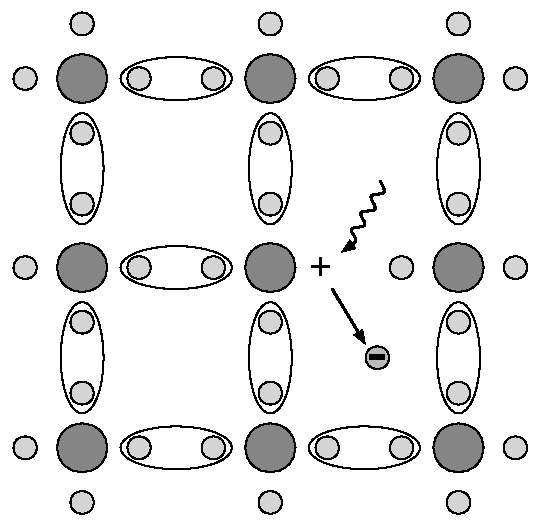
\includegraphics[width=0.4\linewidth]{02_pulse_formation/pics/plots/semilattice9}
%\caption{Valence bonds in the crystalline structure can be broken, producing a free electron-hole pair}
%\label{fig:semilattice9}
%\end{center}
%\end{figure}



The electrons need to absorb a certain energy to get kicked out of the atomic bond -- to get ionised. The minimal energy required to excite (ionise) an electron in a semiconductor is equal to the energy gap $E_\mathrm{g}$. Typical widths of the forbidden gap are 0.7~eV in Ge, 1.12~eV in Si, 1.4~eV in GaAs and 5.5~eV in Di. Due to the small band gap in semiconductors some electrons already occupy the conduction band at room temperature (RT). The intrinsic carrier concentration $n_\mathrm{i}$ in semiconductors is given as
\begin{equation}
\label{eq:intrinsiccarrier}
n_\mathrm{i} = T^{3/2} \cdot exp(-\frac{E_\mathrm{g}}{2kT}) 
\end{equation} 
wherein $k = 1.381\times10^{-23}~$m$^2~$kg~s$^{-2}~$K$^{-1}$ is the Boltzmann constant and T is the temperature. 
%CONTINEUE 

If an external electric field is applied to the crystalline structure, the free electrons and holes drift toward the positive and negative potential, respectively (see figure~\ref{fig:simpledrift}). While drifting, the charges couple with the electrodes, inducing current in the circuit, which is explained by the Shockley--Ramo theorem (see subsection below). The charges recombine upon reaching the electrodes.

\begin{figure}[!t]
\begin{tabular}{cccc}
\subfloat[Valence bonds in the crystalline structure can be broken, creating a free electron-hole pair]{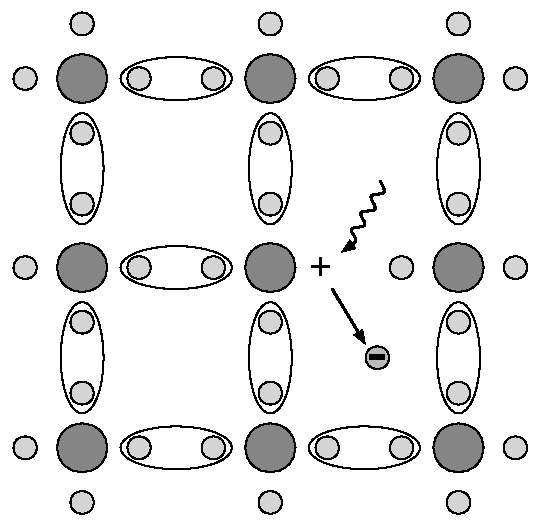
\includegraphics[width=0.22\textwidth]{02_pulse_formation/pics/plots/semilattice9} \label{fig:semilattice9}} &
\subfloat&
\subfloat[The freed electron-hole pair starts drifting in the externally applied electric field. The electron and hole drift in the opposite directions towards the oppositely charged electrods]{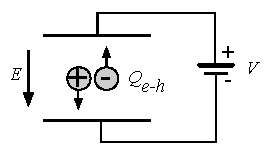
\includegraphics[width=0.33\textwidth]{02_pulse_formation/pics/plots/simpledrift} \label{fig:simpledrift}} &
\subfloat[Equivalent electrical circuit. The moving charges act as a current source]{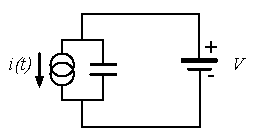
\includegraphics[width=0.33\textwidth]{02_pulse_formation/pics/plots/simpledrifteq}  \label{fig:simpledrifteq}}
\end{tabular}
\caption{In the equivalent electrical circuit diagram, electron-hole creation and drift can be modelled as a current source with a capacitor in parallel }
\end{figure}



%BETHE-BLOCH
\begin{description}
\item[Energy deposition of $\upalpha$ radiation and heavy ions]
\item[Energy deposition of  $\upbeta$ and $\upgamma$ radiation] The mean energy loss of a particle traversing the detector with respect to its momentum is given with the the Bethe-Bloch equation~\cite{}: 
\begin{equation}
-\left\langle\frac{dE}{dx}\right\rangle = \frac{4\pi}{m_\mathrm{e}c^2}  \cdot \frac{nz^2}{\beta^2}  \cdot  \left(\frac{e^2}{4\pi\epsilon_\mathrm{0}}\right)^2  \cdot  \left[ ln \left(\frac{2m_\mathrm{e}c^2\beta^2}{I\cdot(1-\beta^2)}\right)-\beta^2  \right]
\label{eq:bethebloch}
\end{equation}
The resulting function for a muon (a heavy electron) is shown in figure~\ref{fig:bb2}. At the momentum of around 300~MeV/c the particle deposits the lowest amount of energy. That is called a minimum ionising particle or a MIP.
\end{description}


\begin{figure}[!t]
\begin{center}
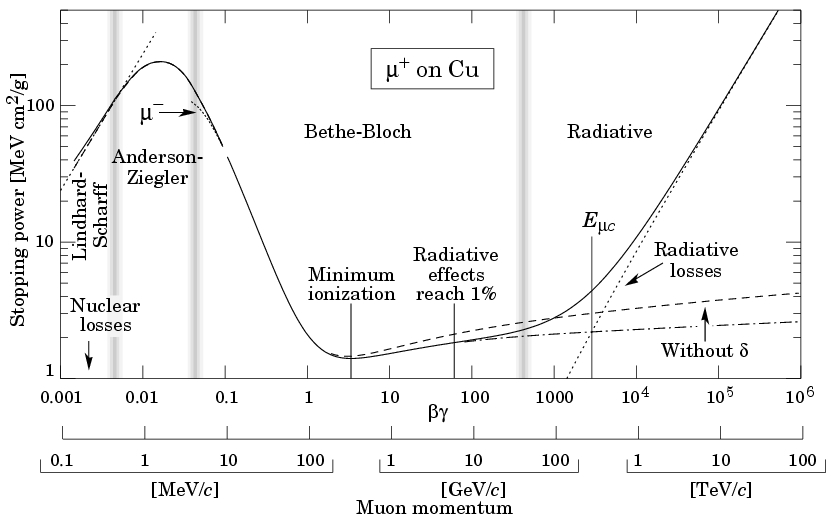
\includegraphics[width=0.85\linewidth]{02_pulse_formation/pics/bb2}
\caption{Stopping power for muons according to the Bethe-Bloch formula~\cite{}}
\label{fig:bb2}
\end{center}
\end{figure}


%Shockley-Ramo theorem
\subsection{Signal induction by moving charges}
The book~\cite{PDDC:00000} gives a simple introduction to understanding signal induction in a conducting plane by a point-like charge. The idea behind it lies in the coupling of the charge with the electrode. The electrode can be in this case modelled as an infinite conducting plane. When the point charge $q$ is created (e.g. an electron-hole pair created via ionisation), its electrostatic field lines immediately couple with the electrode, as seen in figure~\ref{fig:chargeind1}. The electric field on the metal surface due to a point-like charge $q$ at the distance $z_\mathrm{0}$ equals
\begin{equation}
E_\mathrm{z}(x,y) = \frac{qz_\mathrm{0}}{2\pi\epsilon_\mathrm{0}(x^2+y^2+z_0^2)^\frac{3}{2}}~~~~~~~~~~E_\mathrm{y} = E_\mathrm{z} = 0.
\end{equation}
\begin{figure}[!t]
%\centering
\begin{tabular}{cccc}
\subfloat[Newly created point charge couples with the conductive plane]{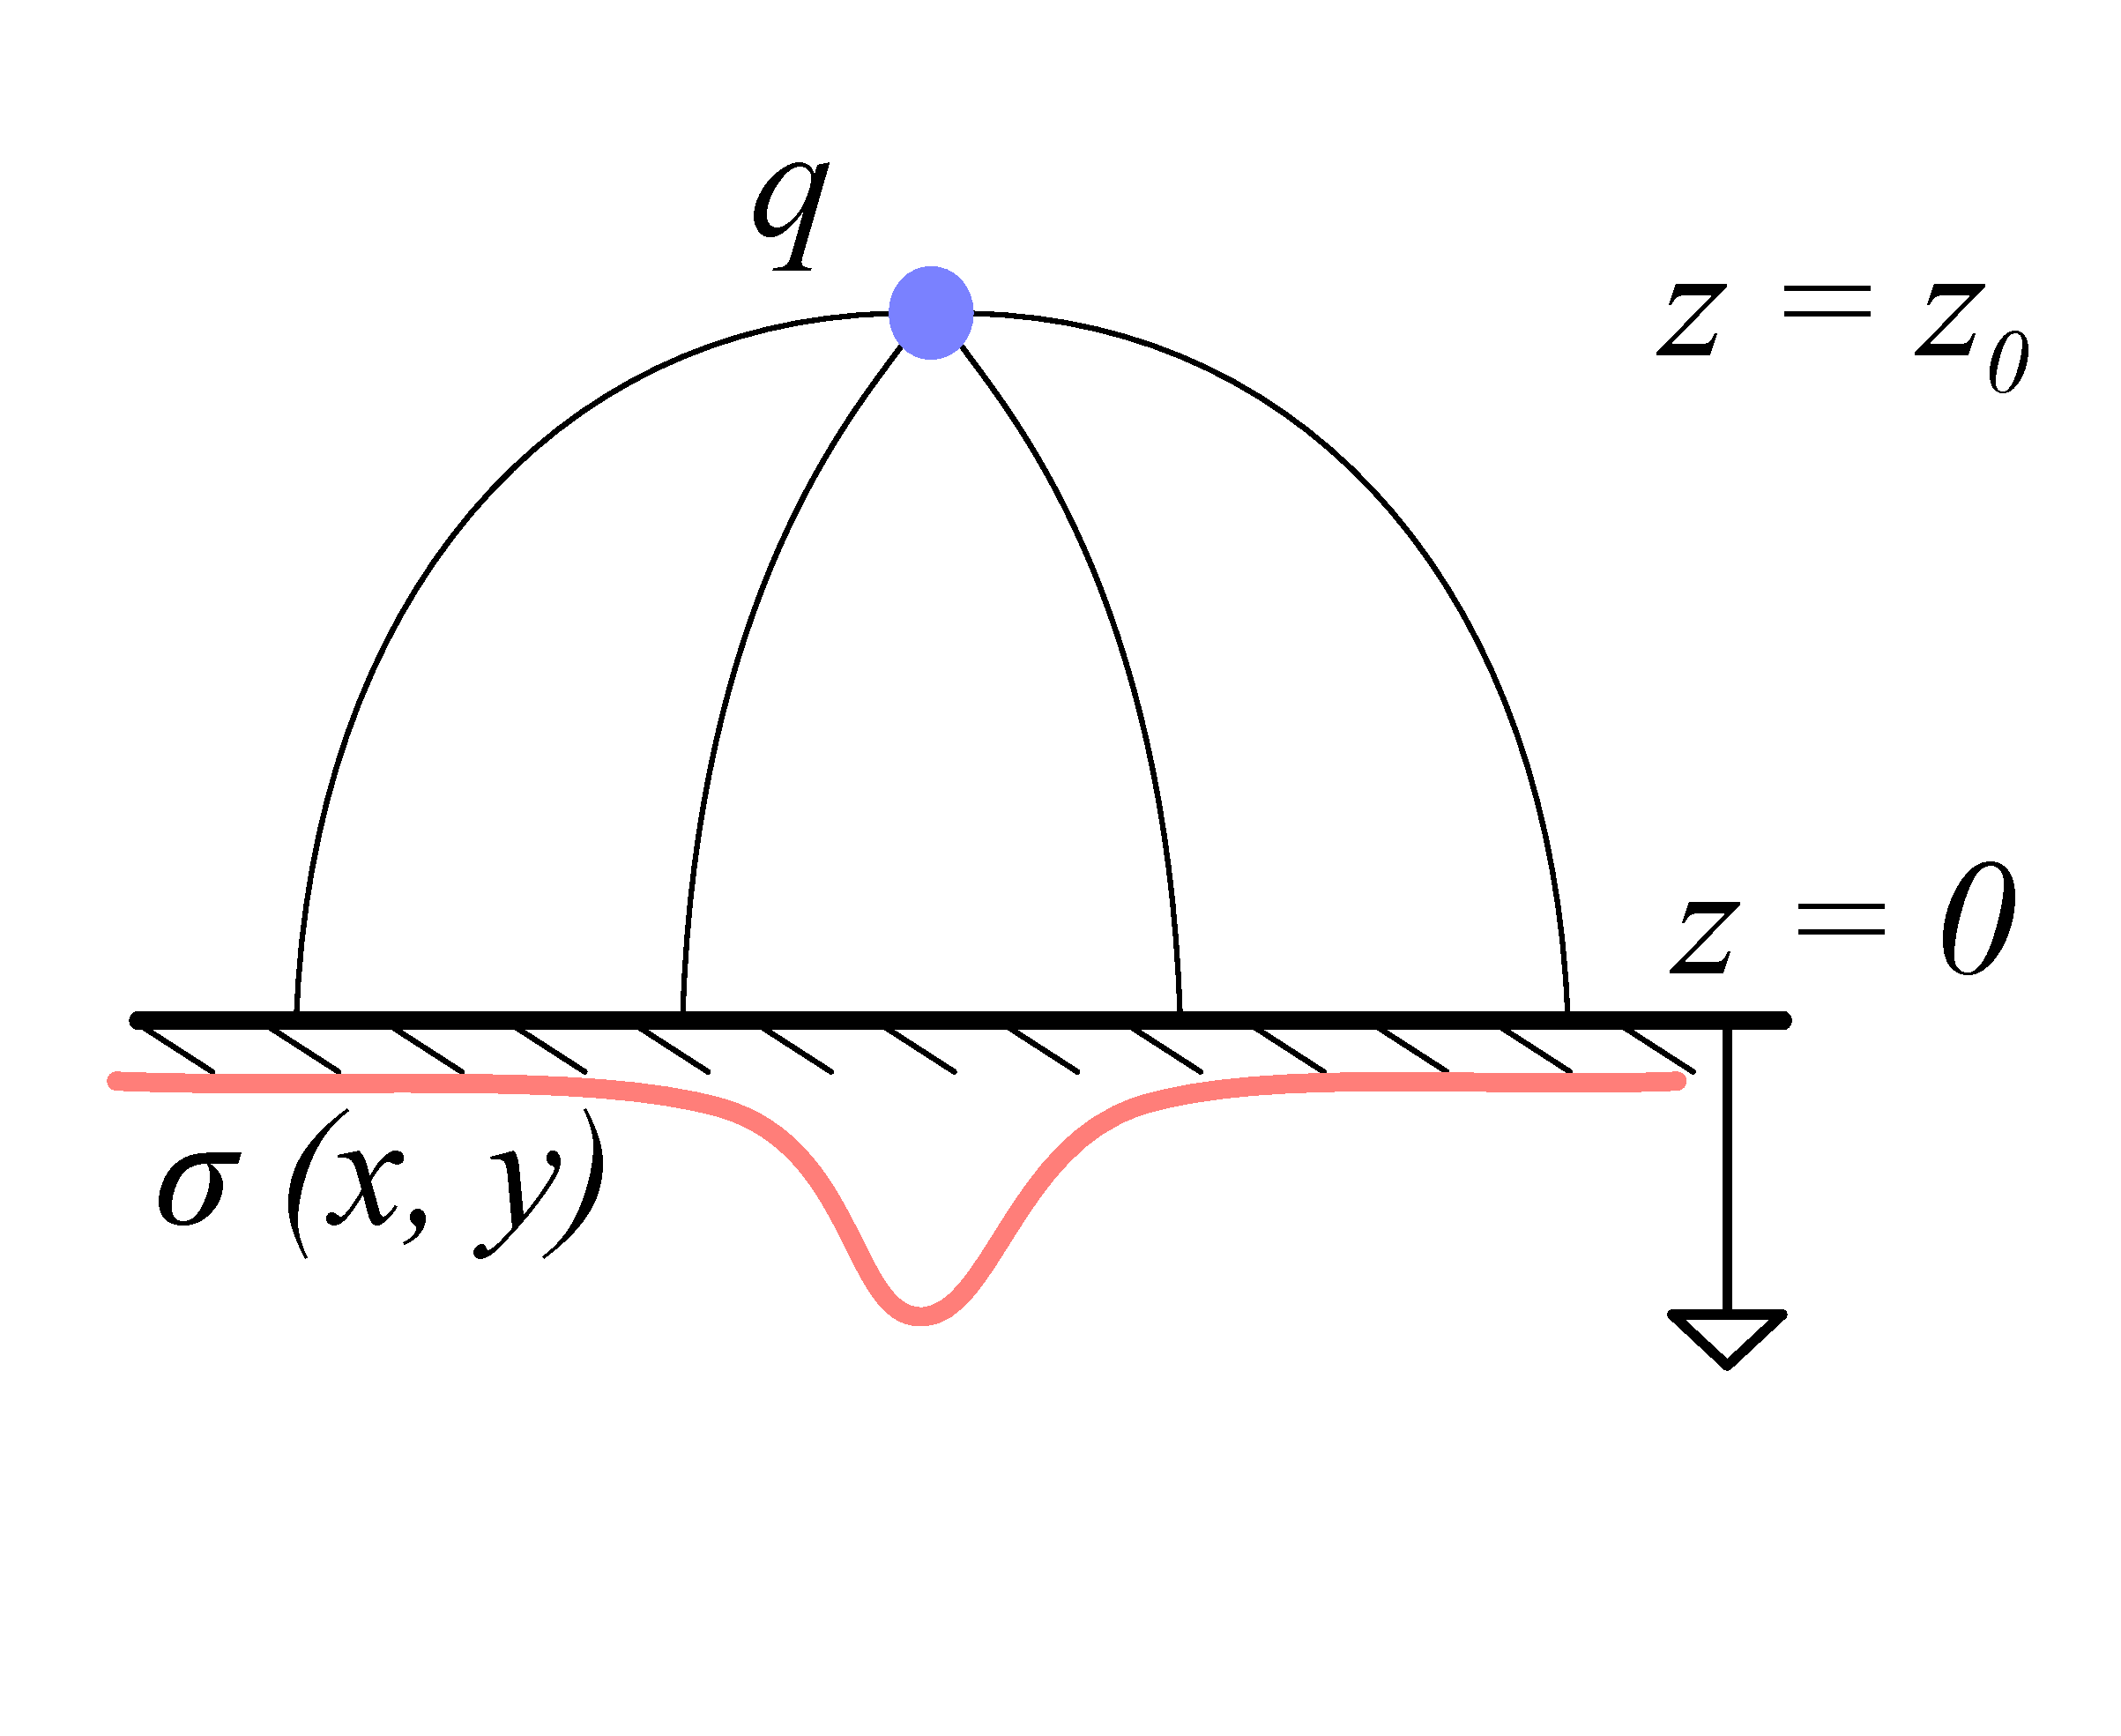
\includegraphics[width=0.30\textwidth]{02_pulse_formation/pics/plots/chargeind1} \label{fig:chargeind1}} &
\subfloat[When the charge drifts, the charge density in the plane changes]{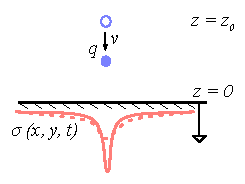
\includegraphics[width=0.30\textwidth]{02_pulse_formation/pics/plots/chargeind2} \label{fig:chargeind2}} &
\subfloat[The changing charge density in the small regions of the plane induces current]{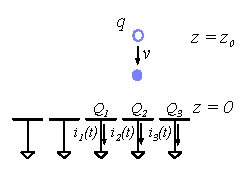
\includegraphics[width=0.30\textwidth]{02_pulse_formation/pics/plots/chargeind3}  \label{fig:chargeind3}}
\end{tabular}
\caption{A point-like charge inducing current in a conductive plane}
\end{figure}
A mirror charge appears on the conducting plane, with a charge density distribution
\begin{equation}
\label{eq:chgdnstydist}
\sigma(x,y)=\epsilon_\mathrm{0}E_\mathrm{z}(x,y)=\frac{qz_\mathrm{0}}{2\pi(x^2+y^2+z_0^2)^\frac{3}{2}}.
\end{equation}
The charge density integrated over the whole plane gives the mirror charge $Q$, which has the opposite value of the point charge $q$:
\begin{equation}
\label{eq:chargedensity}
Q=\int_{-\infty}^{\infty} \int_{-\infty}^{\infty} \sigma(x,y)dxdy = -q.
\end{equation}
Now we segment the plane into infinitely long strips with a width $w$ whereby each of the strips is grounded (figure~\ref{fig:chargeind3}). With the charge density distribution~\ref{eq:chgdnstydist}, the resulting mirror charge on a single strip $Q_\mathrm{2}$ directly below the point charge $(x=0, y=0)$ will be equal to
\begin{equation}
\label{eq:stripcharge}
Q_\mathrm{2}(z_\mathrm{0})=\int_{-\infty}^{\infty}\int_{-w/2}^{w/2}\sigma(x,y)dxdy = -\frac{2q}{\pi}arctan\left(\frac{w}{2z_\mathrm{0}}\right)
\end{equation} 
If the charge starts moving towards the conducting plane, the mirror charge density distribution also changes (see figure~\ref{fig:chargeind2}). This results in the $Q_2[z_0(t)]$ to change with time, inducing an electric current $i_n(t)$:
 \begin{equation}
 \label{eq:indcurr}
 i_n(t) = -\frac{d}{dt}Q_\mathrm{2}[z_\mathrm{0}(t)] = -\frac{\partial Q_\mathrm{2}[z_\mathrm{0}(t)]}{\partial z_\mathrm{0}}\frac{\partial z_\mathrm{0}(t)}{\partial t} = \frac{4qw}{\pi[4z_\mathrm{0}(t)^2 + w^2]}v. 
 \end{equation}
 The movement of the point-like charge therefore induces current in the conducting plane. The induced current is linearly dependent on the velocity of the point-like charge.

W. Shockley~\cite{SHOCKLEY:00000} and S. Ramo~\cite{RAMO:00000} independently proposed a theory which explains how a moving point charge induces current in a conductor. The Shockley-Ramo theorem can therefore be used to calculate the instantaneous electric current induced by the charge carrier or a group of charge carriers. It can be used for any number of electrodes. It states that the current $I_\mathrm{n}^{\mathrm{ind}}(t)$ induced on the grounded electrode $n$ by a point charge $q$ moving along a trajectory $\textbf{x}(t)$ equals
\begin{equation}
\label{eq:ramo}
I_\mathrm{n}^{\mathrm{ind}}(t) = -\frac{dQ_\mathrm{n}(t)}{dt} =  -\frac{q}{V_\mathrm{w}}\nabla\Psi_\mathrm{n}[\textbf{x}(t)]v(t)  =  -\frac{q}{V_\mathrm{w}}E_\mathrm{n}[\textbf{x}(t)]v(t),
\end{equation}
where $\textbf{E}_\mathrm{n}(\textbf{x})$ is the electric field in the case where the charge q is removed, electrode $n$ is  set to voltage $V_\mathrm{w}=1$ and all other electrodes are grounded. $\textbf{E}_\mathrm{n}(\textbf{x})$ is also called the \emph{weighting field} of electrode $n$ and is defined as the spatial differential of the \emph{weighting potential}: $\textbf{E}_\mathrm{n}(\textbf{x})=\nabla \Psi_\mathrm{n}(\textbf{x})$. In the case of two parallel electrodes, the weighting field is $E_\mathrm{w} = -\frac{d\Psi}{dx} = -1/d$, where $d$ is the distance between the electrodes. The resulting induced current is therefore
\begin{equation}
\label{eq:ramoparallel}
i(t) = \frac{q}{d}v_\mathrm{drift}(x,t),
\end{equation} 
whereby $v_{\mathrm{drift}}$ is the drift velocity of the point-like charge and $d$ is the distance between the electrodes.


%moving charge->changed i

%shortened derivation

%i=e/vd


%The energy from an incoming particle can be absorbed by lattice excitation (phonon production) or by ionisation (formation of a mobile charge pair). For a single event, the deposited energy E$_{0}$ is equal to the sum of the energies going into excitation (E$_{ex}$) and ionisation (E$_{ion}$)
%\begin{equation}
%\label{eq:excitationionisation}
%E_0 = E_{ex} N_{ex} + E_{ion} N_{ion}
%\end{equation} 
%where N$_{ex}$ is the number of excitations (phonos produced) and N$_Q$ is the number of charge pairs released. For this event, if more 


\subsection{Radiation-induced electrical pulses}
\begin{figure}[!t]
\begin{center}
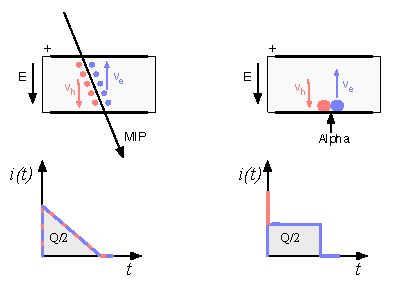
\includegraphics[width=0.8\linewidth]{02_pulse_formation/pics/plots/driftboth}
\caption{Charge carrier drift in diamond for $\upbeta/\upgamma$ and for $\upalpha$ particles}
\label{fig:drift}
\end{center}
\end{figure}When a highly-energetic particle travels through the sensor, it interacts with atoms in the lattice. It ionises the valence electrons, creating electron-hole (e-h) pairs on its way. It can either deposit only a fraction of its energy and fly exit the sensor on the other side or it can get stopped in the bulk, depositing all of its energy. A special case is when it interacts with the core of the atom in the middle of the sensor via a nuclear interaction. All these various types interactions produce different amounts and different spatial distributions of e-h pairs. The induced electrical current will therefore differ for different types of interaction. Two most frequent types are shown in figure~\ref{fig:drift}. The first diagram shows the interaction of a minimum ionising particle (an electron or a proton) or in some cases a photon, if it is energetic enough. The electrons and holes are created all along the trajectory of the particle and immediately start drifting towards the positive and negative electrode, respectively. At the beginning, all charges drift and contribute to the induced current. Those closest to the electrodes have a very short drift path and recombine quickly, reducing the induced current. Gradually all the charge carriers recombine. The resulting current signal is a triangular pulse with a sharp rising edge and a linear falling edge. The accumulated charge $Q_\mathrm{s}$ equals to the sum of the contributions of the positive and negative charge carriers. The second type of interaction happens when the particle is stopped in the diamond close to the point of entry. Most of its energy is deposited in a small volume close to the electrode. A cloud of charge carriers is created and the charges with the shorter path to the electrode recombine almost instantly. The carriers of the opposite charge, however, start drifting through the sensor to the other electrode. In an ideal diamond sensor, their velocity is constant throughout the drift up until they recombine on the other side. The contribution of the first charge cloud is a peak with a short time. The cloud drifting through the sensor, on the other hand, induces a current signal with a flat top. The resulting signal has a shape of a rectangle, with a spike in the beginning. This spike is filtered out in a real device because it is too fast for the electronics existing currently. The accumulated charge $Q_\mathrm{s}$ is equal to a half of the deposited charge by the stopped particle.

The two aforementioned types of interactions have well defined signal responses. Nuclear interactions on the other hand yield various results. The resulting signal shape depends on the decay products of the interaction -- they can be $\upalpha$, $\upbeta$ or $\upgamma$ quanta, inducing a mixed shaped signal. 
%
%Current profiles
%Alpha
%beta
%gamma
%neutron


\subsection{Signal charge fluctuations}
Two of the important sensor characteristics are the magnitude of the signal and the fluctuations of the signal at a given absorbed energy. They determine the relative resolution $\Updelta E/E$. For semiconductors the signal fluctuations are smaller than the simple statistical variance $\upsigma_\mathrm{Q}=\sqrt{N_\mathrm{Q}}$, where $N_\mathrm{Q}$ is the number of released charge pairs (ratio between the total deposited energy $E_\mathrm{0}$ and the average energy deposition $E_\mathrm{i}$ required to produce an electron-hole pair). \cite{} shows that the variance is $\upsigma_\mathrm{Q}=\sqrt{F N_\mathrm{Q}}$, where $F$ is the Fano factor~\cite{} (0.08 for diamond and 0.115 for silicon ~\cite{}). Thus, the variance of the signal charge is smaller than expected, $\upsigma_\mathrm{Q}\approx0.3 \sqrt{N_\mathrm{Q}}$. The resulting intrinsic resolution of semiconductor detectors is 
\begin{equation}
\label{eq:efwhm}
\Updelta E_{FWHM} = 2.35 \sqrt{FEE_\mathrm{i}} 
\end{equation} 
wherein $E_\mathrm{i}(Si)$=~3.6~eV and E$_\mathrm{i}(C)$=~13~eV. E.g., for an $\upalpha$ particle with energy $E_\upalpha$ = 5.486 MeV the calculated resolution in diamond is equal to $\Updelta E_{\mathrm{FWHM}}$ = 5.6~keV. This defines the maximum achievable resolution for energy spectroscopy with semiconductors. Figure~\ref{fig:enerres} shows the calculated energy resolution function for silicon and diamond.

\begin{figure}[!t]
\begin{center}
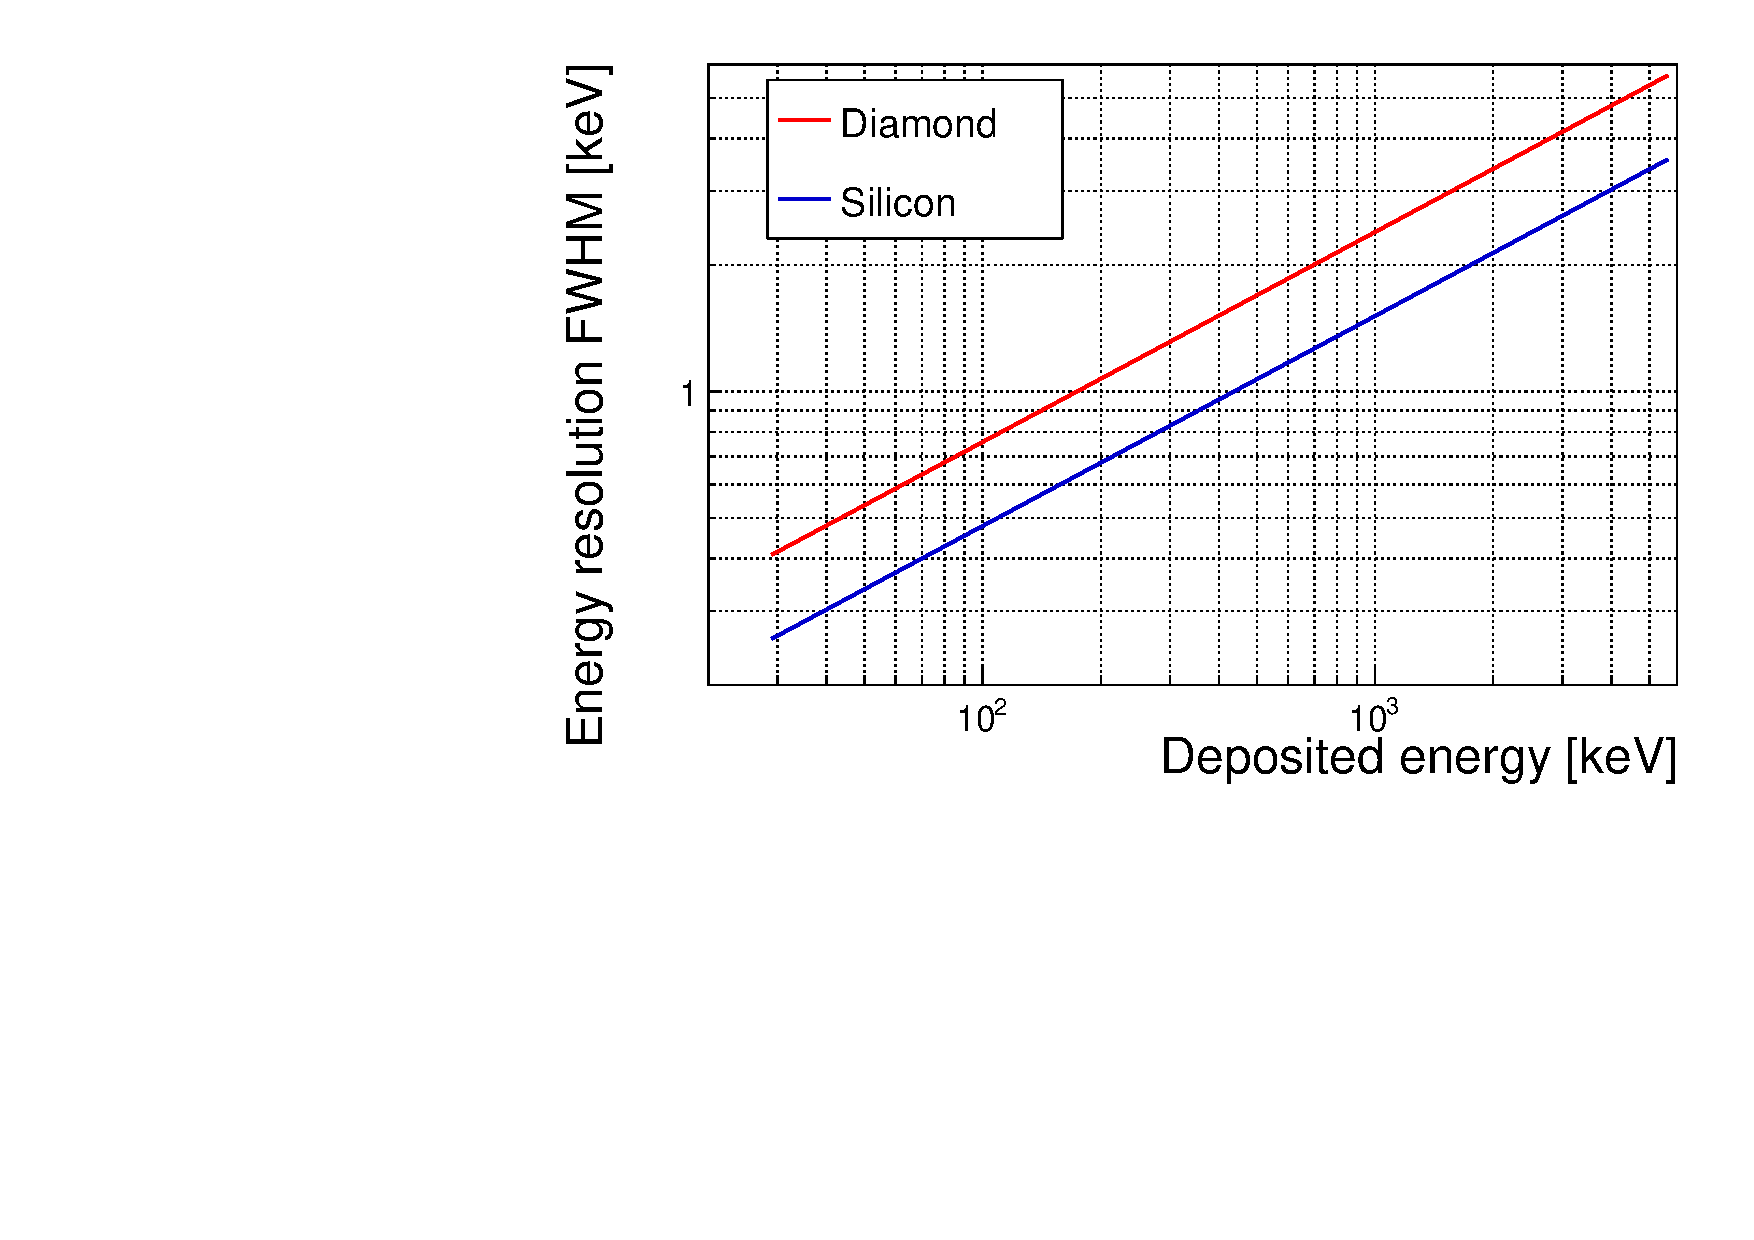
\includegraphics[width=0.8\linewidth]{../scripts/02_pulse_formation/plots/resolution}
\caption{Calculated intrinsic energy resolution for silicon and diamond}
\label{fig:enerres}
\end{center}
\end{figure}




% ---------------------------------------------------------------------------------------------------------------
%\clearpage
\section{Carrier transport in a diamond sensor} 
% ---------------------------------------------------------------------------------------------------------------
This section describes the carrier transport phenomena in diamond. This theory provides the basis for discussion about the measurements in chapter~\ref{ch:meas}. 

Free charge carriers in a semiconductor get thermally excited and scatter in random directions with a thermal velocity $v_{\mathrm{th}}$~\cite{}. Their integral movement due to thermal excitation equals zero. Their transport is instead by means of drift and diffusion. Diffusion is caused by the concentration gradient. In its presence the carriers tend to scatter in the direction of the lower concentration. Drift on the other hand is caused by an externally applied electrical field. In that case the carriers move in parallel to to the field lines. In a sensor with a high applied field the diffusion contribution is negligible. 

\begin{description}

\item[Diffusion]
The concentration profile dissolves with time forming a Gaussian distribution with variance $\sigma(t)=\sqrt{Dt}$~\cite{} .

\item[Drift velocity and mobility]
The charge carriers drift through the diamond bulk with a drift velocity $v_\mathrm{drift}(E)$~\cite{}, which is proportional to the electric field $E$ at low electric fields: $v_\mathrm{drift} = \mu E$. The proportionality factor $\mu$ is defined as the mobility in cm$^2$V$^{-1}$s$^{-1}$. For higher fields, however, the velocity saturates. The final equation for $v_\mathrm{drift}$ is therefore
\begin{equation}
\label{eq:vsat}
v_\mathrm{drift}(E) = \mu(E)E= \frac{\mu_\mathrm{0} E}{1 + \frac{\mu_\mathrm{o} E}{v_\mathrm{sat}}}
\end{equation}
where $\mu_\mathrm{0}$ is the low field mobility and $v_\mathrm{sat}$ is saturation velocity. The drift velocity can be retrieved experimentally via the transit time measured with the Transient Current Technique (TCT). This technique enables the measurement of transit time $t_\mathrm{t}$ of the carriers through the sensor with the thickness $d$. 
\begin{equation}
\label{eq:vsat}
v_\mathrm{drift}(E) = \frac{d}{t_\mathrm{t}(E)}.
\end{equation}
The velocities for holes and electrons usually differ. In diamond, the holes travel 30~\% faster than electrons~\cite{}. The measurements in chapter~\ref{ch:meas} empirically confirm this statement.

\item[Velocity saturation] At higher drift velocities the carriers lose more energy to the lattice. They induce increasingly more lattice vibrations (phonon transport) with increased velocity. There is a velocity limit above which the carriers cannot reach -- velocity saturation. Thesis~\cite{} defines this velocity to be $v^e_\mathrm{sat}=v^h_\mathrm{sat}=(14.23\pm0.12)\times10^6$~cm/s for both positive and negative charge carriers.

\item[Space carge] 
Poisson's equation shows that 
\begin{equation}
\label{eq:poisson}
\frac{d^2\Phi(x)}{dx^2} = \frac{dE(x)}{dx} = \frac{\rho(x)}{\epsilon}
\end{equation}
where $\rho(x)$ is the space charge distribution, $E$ is the electrical field and $\Phi$ is the voltage potential. In an ideal diamond, the externally applied high voltage potential on the two electrodes decreases linearly through the bulk. The electrical field is therefore constant throughout the sensor and the space charge distribution across it equals 0. However, in some cases space charge is introduced in the bulk, uniformly or non-uniformly. It can do so by means of trapping of charge carriers in the non-uniformities in the lattice or it can already be introduced during the production of the diamond material. The space charge can be either permanent or changing -- sometimes it is possible to reduce it by means of priming. All in all, it is very important to reduce it because it affects the shape of the electrical signal. Since the drift velocity of the charge carriers is proportional to the electrical field, the charges change their velocity while drifting through the space charge region. Figure~\ref{fig:spcchg} compares the voltage potential, electrical field, space charge for an ideal sensor and for that with a uniformly distributed positive space charge.
\begin{figure}[!t]
\begin{center}
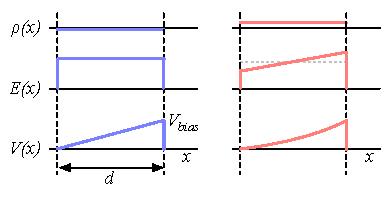
\includegraphics[width=0.6\linewidth]{02_pulse_formation/pics/plots/spcchg}
\caption{Introduction of space charge in the diamond bulk. The induced current signal is proportional to the effective electrical field. $d$ is the thickness of the diamond sensor.}
\label{fig:spcchg}
\end{center}
\end{figure}


\item[Radiation damage]
The diamond crystal lattice is very strong and uniform. However, when the highly energetic particles or photons impinge the diamond, they can damage the crystal structure. Figure~\ref{fig:raddamage} shows several examples of the lattice damage:
\begin{enumerate}
\item[a)]foreign interstitial (e.g. H, Li),
\item[b, c)]foreign substitutional (e.g. N, P, B),
\item[d)]vacancy and
\item[e)]self interstitial.
\end{enumerate} 
These non-uniformities -- traps -- form new energy levels in the forbidden gap. The drifting charge carriers are stopped by these traps, which in effect reduces the induced current. The energy level of the trapped carrier is reduced from the conduction band to the energy level of the trap. Different types of lattice damage have different energy levels. The release time depends on the level (shallow, deep trap).

\begin{figure}[!t]
\begin{center}
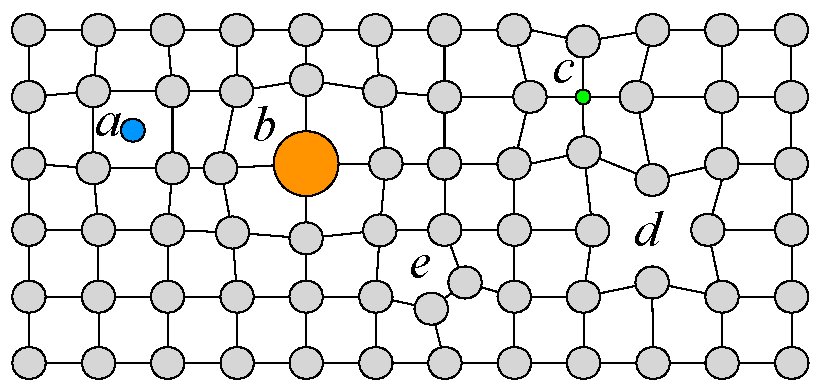
\includegraphics[width=0.8\linewidth]{02_pulse_formation/pics/plots/raddamage}
\caption{Introduction of impurities and non-uniformities into the crystal lattice due to radiation damage.}
\label{fig:spcchg}
\end{center}
\end{figure}

\end{description}













% ---------------------------------------------------------------------------------------------------------------
%\clearpage
\section{Electronics for signal processing} % signal acquisition
% ---------------------------------------------------------------------------------------------------------------
\label{sec:elecsigproc}
This section describes the electronics of a detector, starting with a description of signal amplifiers and then discussing the digitisation and signal processing. All these stages are necessary to extract information from the sensor. First, the signal has to be amplified. Then it is digitised and finally processed in a specially designed processor or a logic unit.

\subsection{Signal preamplifiers}
The signal charge generated in the sensor by a single highly energetic particle or photon is of the order of fC. The induced current is ranging between $10^{-8}$~A ($\upbeta, \upgamma$ radiation) and $3\times10^{-7}$~A ($\upalpha$ radiation). Signals as low as these have to be pre-amplified before processing. Depending on the measurement, several types of signal amplifiers can be used. The preamplifiers have to be designed carefully to minimise electronic noise while maximising gain -- thus maximising the signal-to-noise ratio (SNR). In addition, they have to have a high bandwidth limit because the signals from the diamond sensors are very short. A critical parameter is the total capacitance, i.e. sensor capacitance and input capacitance of the preamplifier. The SNR improves with a lower capacitance. Several types of amplifiers can be used, all of which affect the measured pulse shape. They behave differently for resistive or capacitive sources. Given that semiconductors are capacitive sources, we will focus on these. Two preamplifiers are used most commonly, a current and a charge amplifier. Both are described below in detail. 

\begin{figure}[!t]
%\centering
\begin{tabular}{cccc}
\subfloat[A capacitive source and a current amplifier]{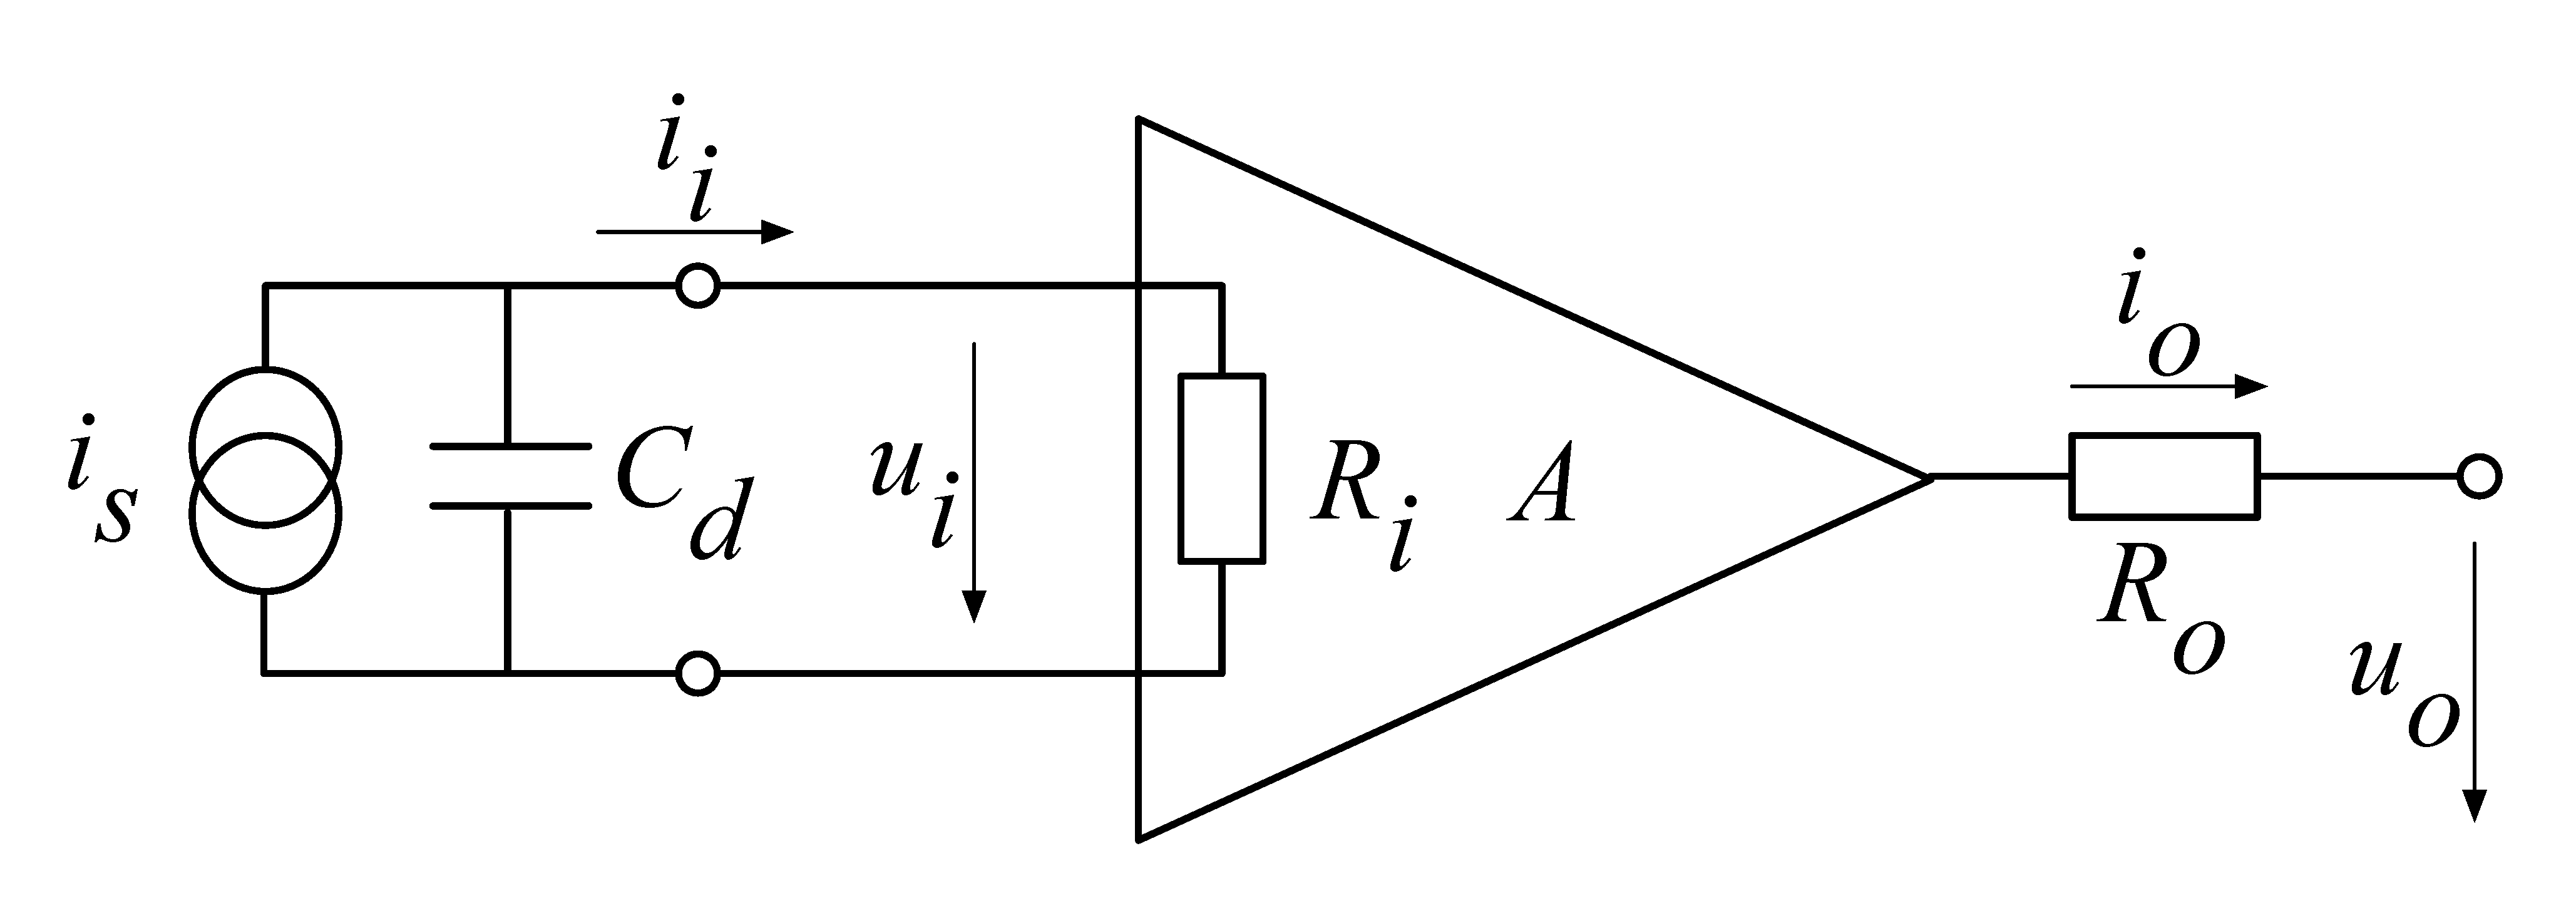
\includegraphics[width=0.50\textwidth]{02_pulse_formation/pics/plots/curramp} \label{fig:curramp}} &
\subfloat[A capacitive source and a charge amplifier]{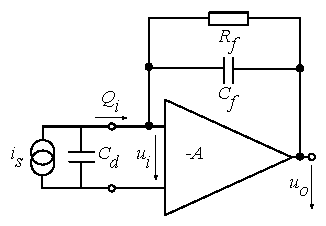
\includegraphics[width=0.40\textwidth]{02_pulse_formation/pics/plots/chgamp}  \label{fig:chgamp}}
\end{tabular}
\caption{Simplified equivalent circuits of a current and charge amplifier }
\end{figure}


\subsubsection{Current-sensitive amplifier}
Figure~\ref{fig:curramp} shows the equivalent circuit of a capacitive source and a current amplifier. An amplifier operates in current mode if the source has a low charge collection time $t_\mathrm{c}$ with respect to the $R_\mathrm{i}C_\mathrm{d}$ time constant of the circuit. In this case the sensor capacitance discharges rapidly and the output current $i_\mathrm{o}$ is proportional to the instantaneous current $i_\mathrm{i}$. The amplifier is providing a voltage gain, so the output signal voltage $u_o$ is directly proportional to the input voltage $u_\mathrm{i}$:
\begin{equation}
u_\mathrm{o}(t) = A \cdot R_\mathrm{i} \cdot i_\mathrm{s}(t).
\end{equation}
The detector capacitance $C_\mathrm{det}$ together with the input resistance of the amplifier $R_\mathrm{i}$ defines the time constant of the signal (see figure~\ref{fig:currc}). The higher the $C_\mathrm{det}$ is, the slower will be the response of the amplifier. For the case of the diamond sensor, which has the capacitance of the order of 2~pF and the input resistance of 50~$\Omega$, the resulting time constant is $\tau=10^{-10}$~s. This yields the signal rise time $t_\mathrm{r}\sim2.2\tau=0.22~ns$.
\begin{figure}[!t]
\begin{center}
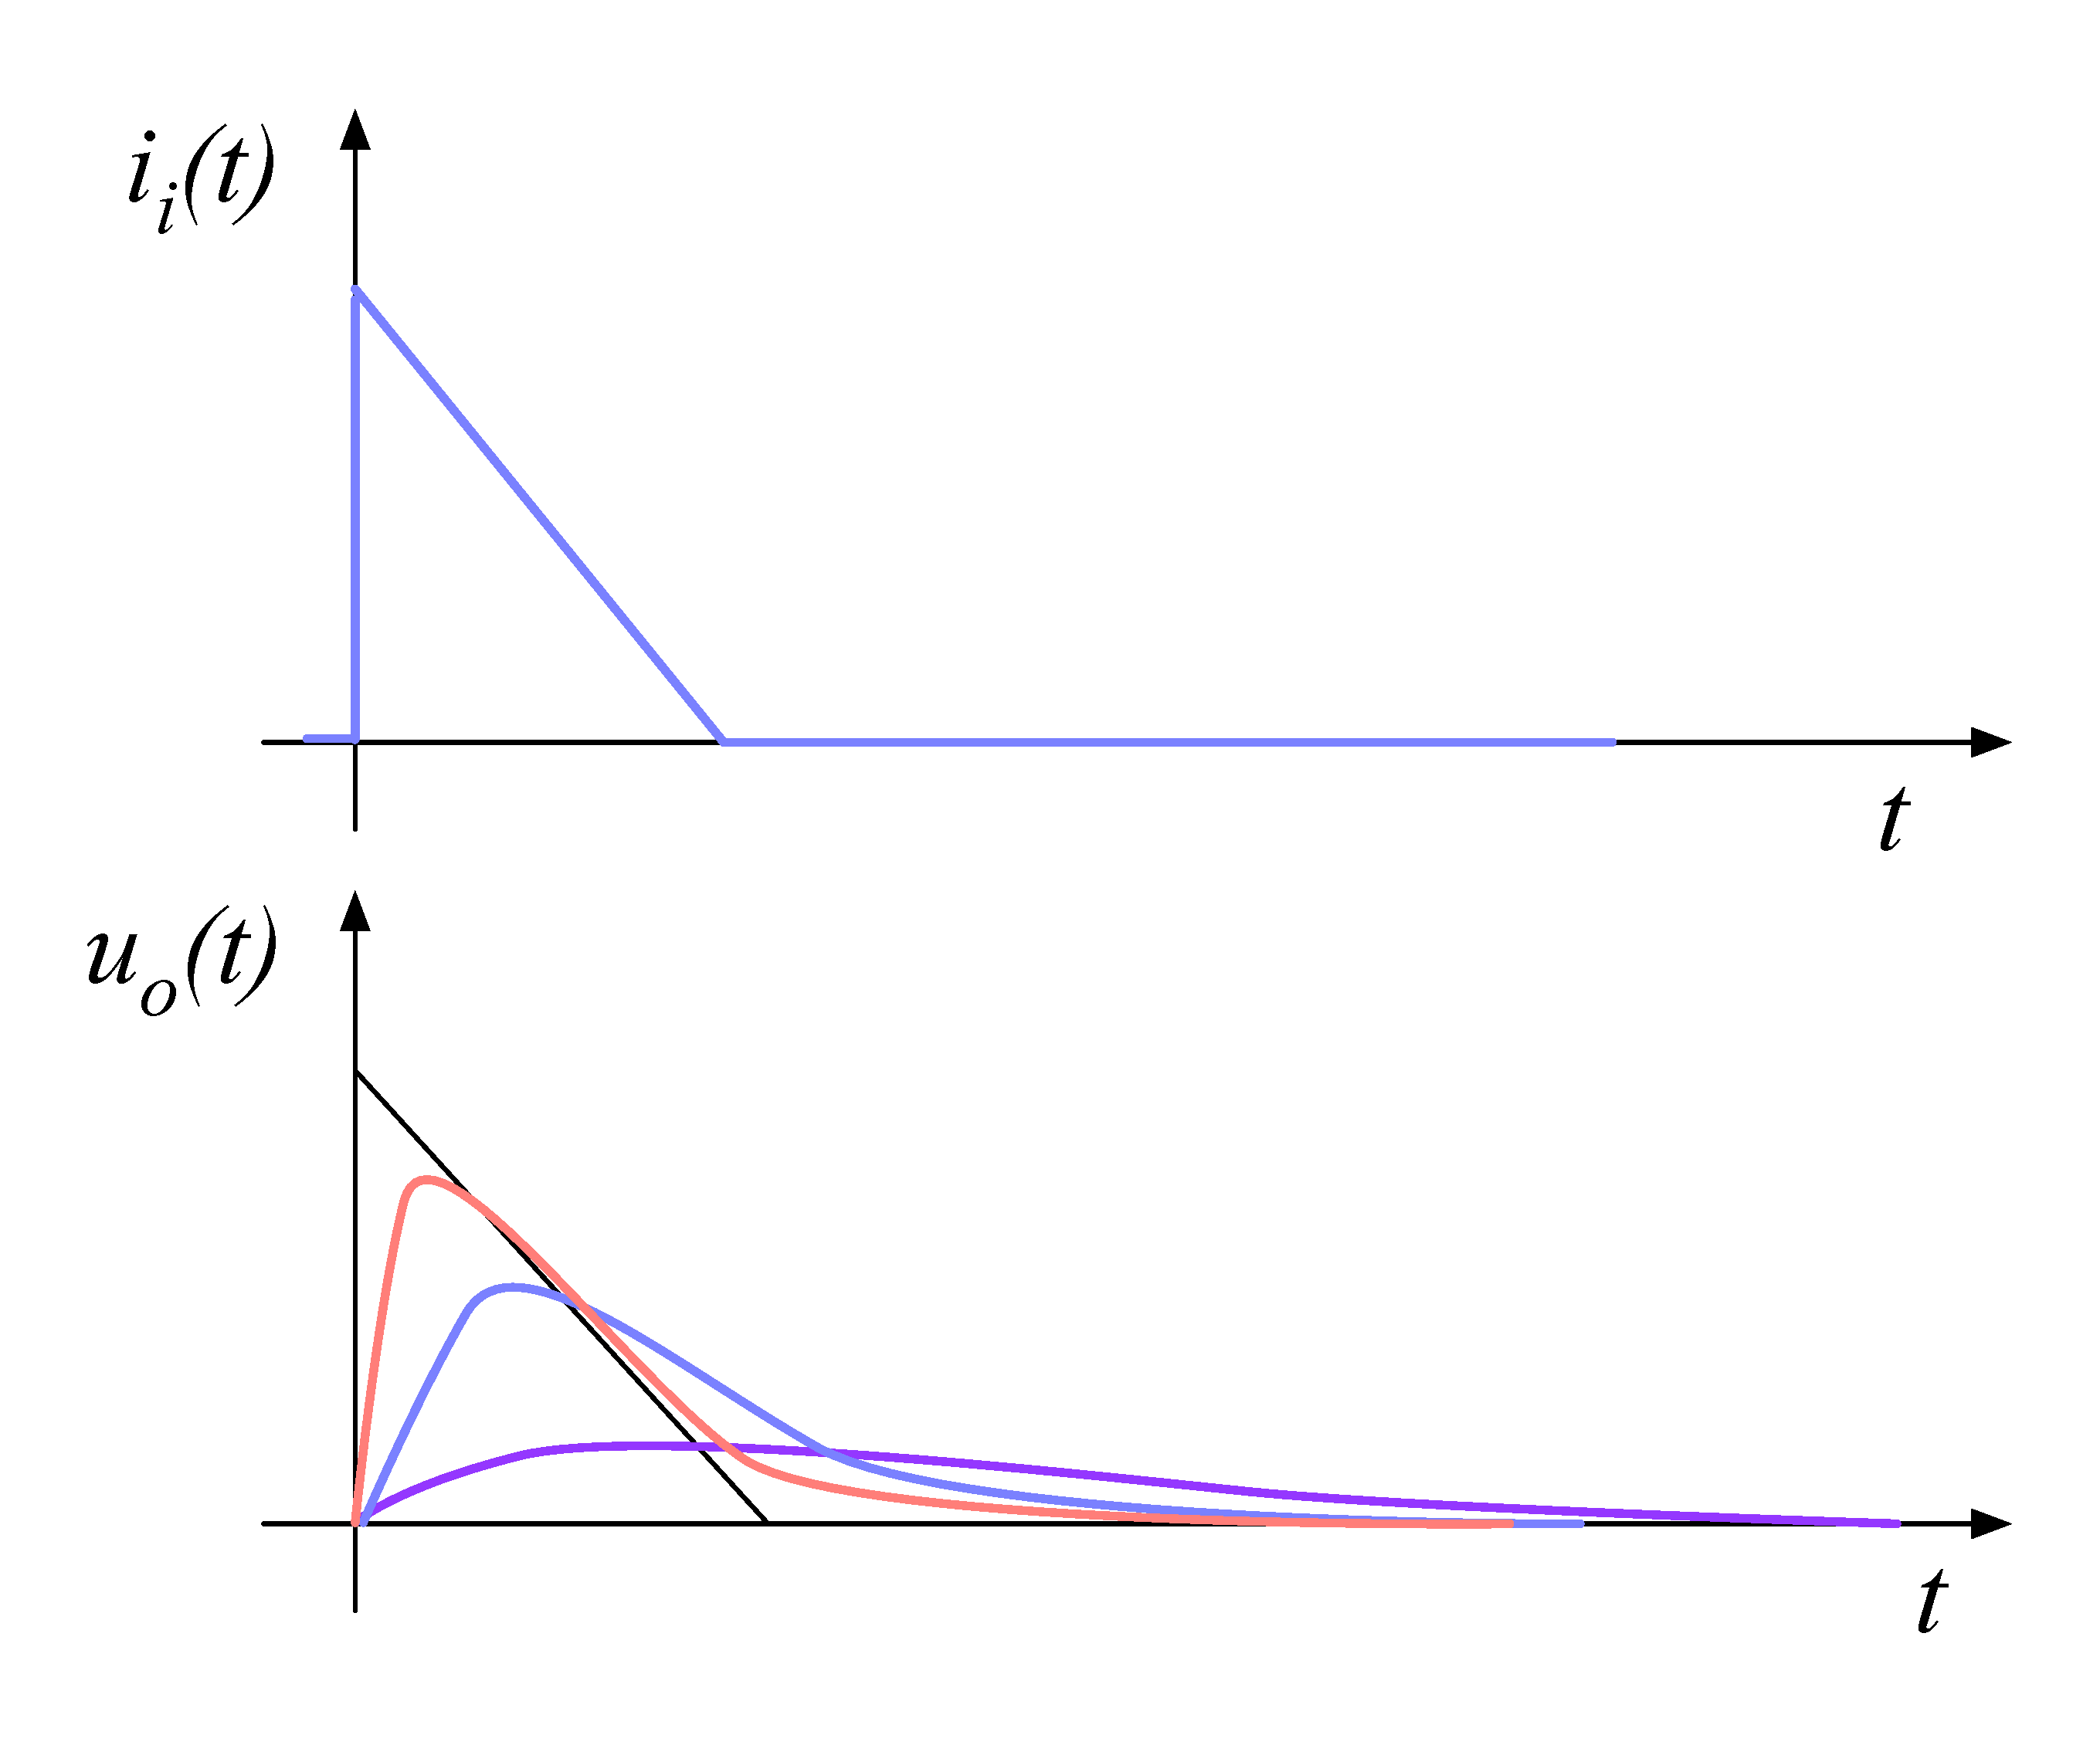
\includegraphics[width=0.8\linewidth]{02_pulse_formation/pics/plots/currrc}
\caption{Input and output signal of the current amplifier}
\label{fig:currc}
\end{center}
\end{figure}




\subsubsection{Charge-sensitive amplifier}
%(0.5 pg)
In order to measure integrated charge in the sensor, a feedback loop is added to the amplifier (see figure~\ref{fig:chgamp}). The feedback can be used to control the gain and input resistance, as well as to integrate the input signal. The charge amplifier is in principle an inverting voltage amplifier with a high input resistance. 
 
In an ideal amplifier the output voltage $u_\mathrm{o}$ equals $-Au_\mathrm{i}$. Therefore the voltage difference across the capacitor $C_\mathrm{f}$ is $u_\mathrm{f}=(A+1)u_\mathrm{i}$ and the charge deposited on the capacitor is $Q_\mathrm{f}=C_\mathrm{f}u_\mathrm{f} = C_\mathrm{f}(A+1)u_\mathrm{i}$. Since no current can flow into the amplifier, all of the signal current must charge up the feedback capacitance, so $Q_\mathrm{f} = Q_\mathrm{i}$.

In reality, however, charge-sensitive amplifiers respond much slower than is the duration of the current pulse from the sensor. In addition, a resistor is added to the feedback line in parallel to the capacitor. The resistor and capacitor define the decay time constant of the pulse (see figure~\ref{fig:chgrc}). This is necessary to return the signal to its initial state and ready for a new measurement.
\begin{figure}[!t]
\begin{center}
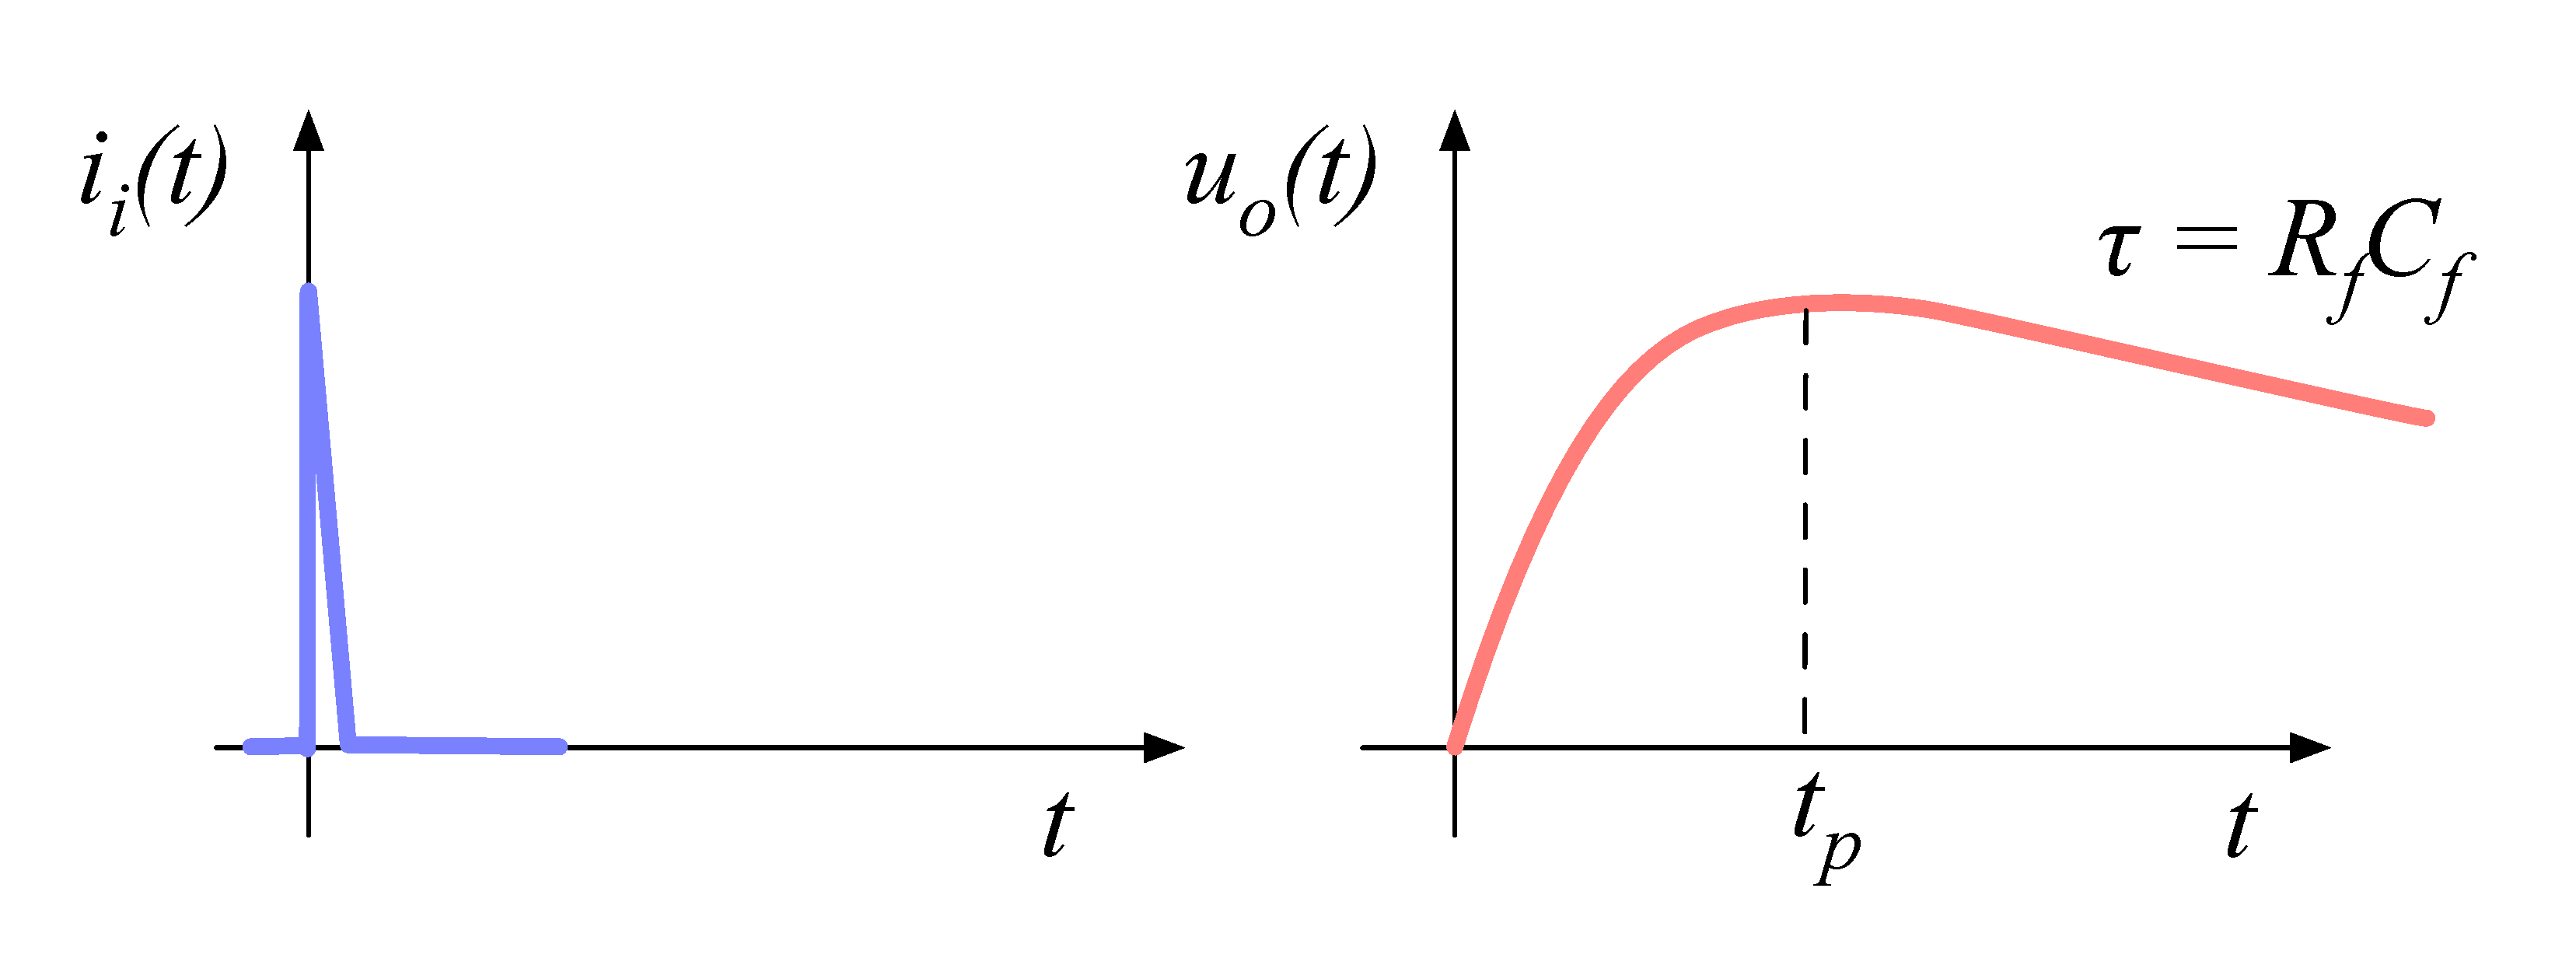
\includegraphics[width=0.7\linewidth]{02_pulse_formation/pics/plots/chgrc}
\caption{Input and output signal of the charge amplifier}
\label{fig:chgrc}
\end{center}
\end{figure}

\subsubsection{Analogue electronic noise}
%(2 pg)
Electronic noise determines the ability of a system to distinguish signal levels. The analogue signal contains a lot of information, which can quickly be erased or altered if the signal properties change. It is therefore instrumental to understand the noise contributions to the signal to qualify the information it carries. There are several noise contributions, of which the important ones are listed below. The thermal noise is the dominant noise contribution in the use case for diamond detector signal amplification and therefore defines the limitations of the detector system. Thermal noise or Johnson--Nyquist~\cite{} noise is generated by the random thermal motion of charge carriers in the conductor. The frequency range of the thermal noise is from 0 to $\infty$ with a more or less uniform distribution. Therefore this is nearly a white noise. The resulting signal amplitude has a Gaussian distribution. The RMS of the noise amplitude is defined as
\begin{equation}
\label{eq:thermnoise}
u_\mathrm{RMS}=\sqrt{4k_BRT\Delta f}
\end{equation}
where $k_\mathrm{B}$ is the Boltzmann constant, $R$ is the resistance of the conductor, $T$ its temperature and $\Delta f$ the frequency range. This equation shows that it is possible to reduce the noise RMS by either (1) reducing the frequency range, (2) reducing the resistance of the conductor or (3) cooling the conductor. 

Contributions of shot noise, flicker noise and burst noise and other types are not significant relative to the thermal noise. However, the contributions of external factors can severely deteriorate the signal. This means the noise produced by capacitive or inductive coupling with an external source, which causes interference in the signal. These effects can be reduced by shielding the electronics and avoiding ground loops. 

\subsection{Analogue-to-digital converters}
An analogue-to-digital converter (ADC) is a device that converts the analogue electrical signal on the input to its digital representation - a series of digital values. This involves a quantisation -- \emph{sampling} of the signal at a defined sampling period, resulting in a sequence of samples at a discrete time period and with discrete amplitude values. The resolution of the ADC is the number of output levels the ADC can quantise to and is expressed in bits. For instance, an ADC with a resolution $n=8$~bit will have the dynamic range $N=2^n=256$~steps. The resulting voltage resolution $Q_\mathrm{ADC}$ at the input voltage range of $V_\mathrm{ADC}=\pm$50~mV is then equal to 
\begin{equation}
\label{eq:mvpercnt}
Q_\mathrm{ADC}=\frac{V_\mathrm{ADC}}{2^{n}}  = \frac{100~mV}{2^8~steps} = 0.39~mV/step.
\end{equation} 
With a sampling period of $t_\mathrm{s}=$1~ns this will produce the sampling rate of $f_\mathrm{s}=$1~GSPS (gigasample per second).
\begin{figure}[!t]
\begin{center}
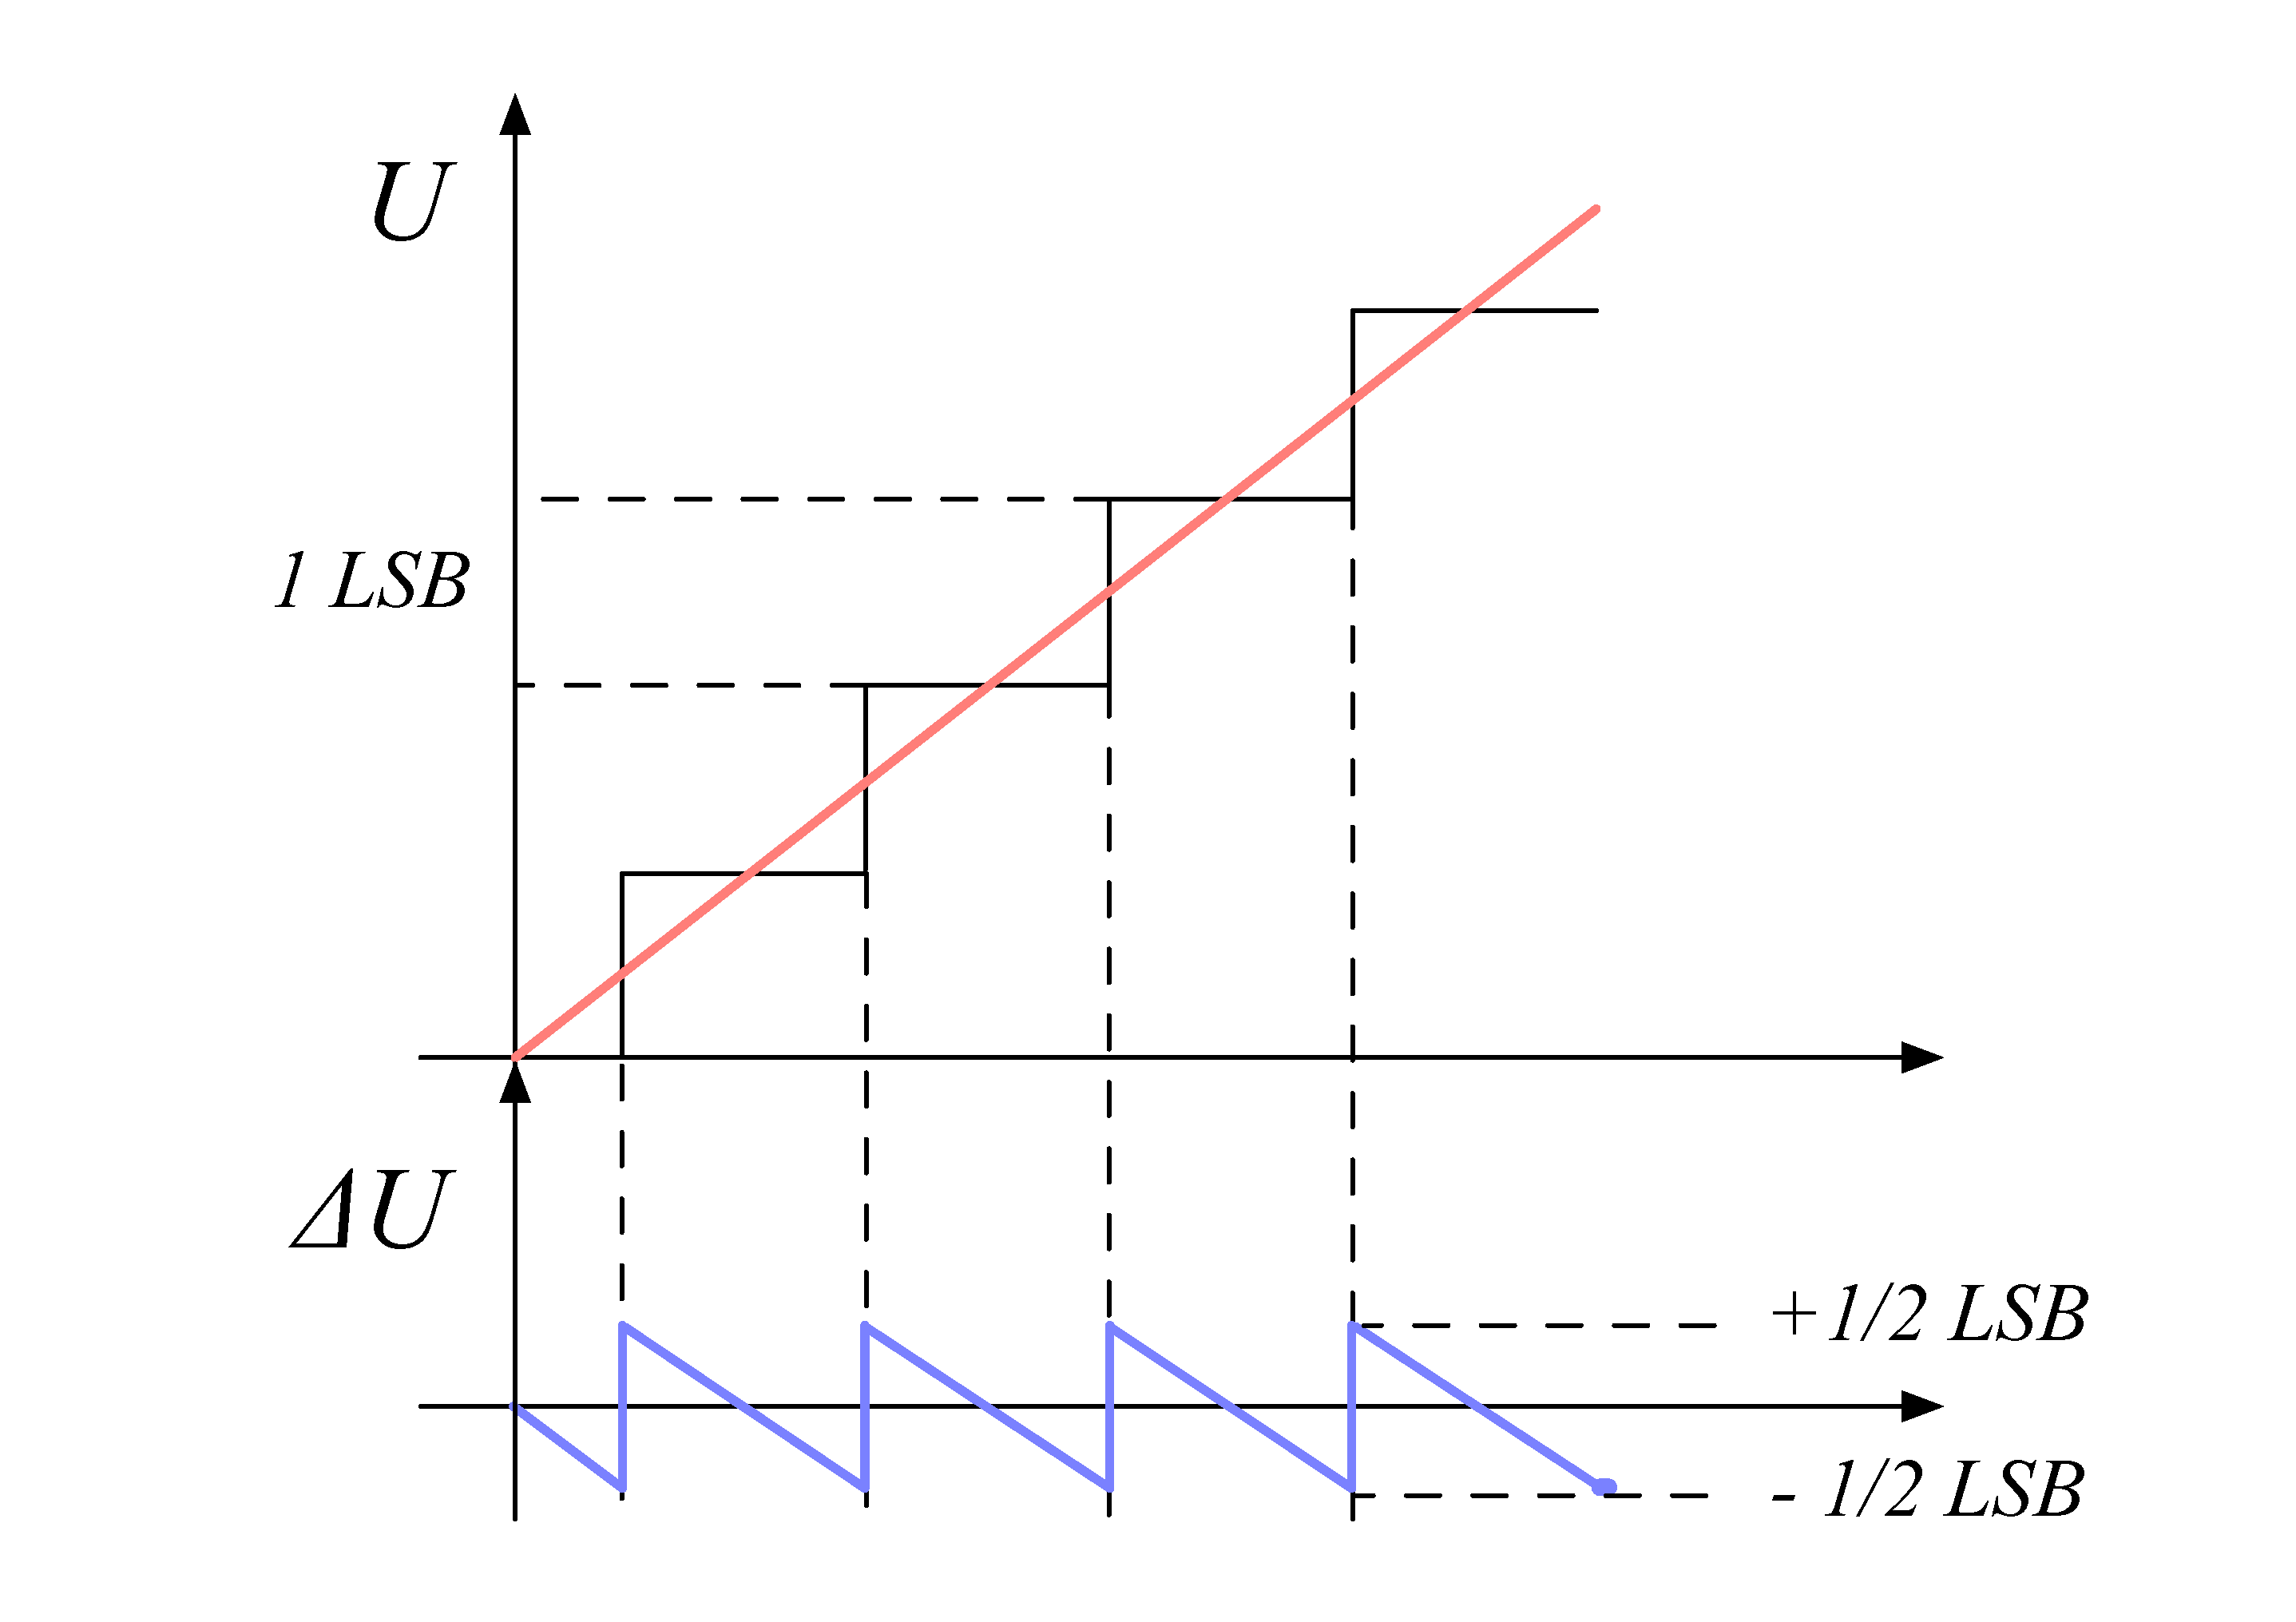
\includegraphics[width=0.7\linewidth]{02_pulse_formation/pics/plots/qerr}
\caption{Input signal digitisation and quantisation error}
\label{fig:qerr}
\end{center}
\end{figure}

\begin{description}
\item[Quantisation error and quantisation noise] (or a round-off error) is a contribution to the overall measurement error due to digitisation (rounding). It is defined as a difference between the actual analog value and a digitised representation of this value. The error is defined by the least significant bit (LSB), as seen in figure~\ref{fig:qerr}. Typically, the input signal amplitude is much larger than than the voltage resolution. Therefore the quantisation error is not directly correlated with the signal and has an approximately uniform distribution~\cite{}: 
\begin{equation}
\label{eq:qerr}
\Delta Q_\mathrm{ADC}=\frac{1}{\sqrt{12}}LSB\sim0.289~LSB.
\end{equation} 
For the example above the quantisation error will be $\Delta Q_\mathrm{ADC}=0.289\cdot 0.39$~mV=0.11~mV. The error depends strongly on the linearity of the ADC, but this will not be discussed in this document as the devices used have ADCs with a linear response.
\end{description}

\subsection{Digital signal processing}
The digitised signal can be processed to extract useful information. Therefore after the signal amplification and digitisation the signal is routed in a device which handles the analysis. The signal can either be processed immediately (in real time) or it can be saved to a data storage for analysis at a later stage (offline). The devices carrying out the processing can be multipurpose (e.g. Field programmable gate arrays) or dedicated (e.g. application-specific integrated circuits). Each of the two has its advantages and disadvantages, which are listed below. 

\begin{description}
\item[Field programmable gate array] (FPGA) is an integrated circuit designed to be reprogrammable and reconfigured after manufacturing. It consists of a set of logic gates that can be interconnected in numerous combinations to carry out a logic operation. Many such logic operations can take place in parallel, making the FPGA a powerful tool for signal processing. FPGAs are often used during system development or in systems in which the requirements might change with time. They can be reprogrammed in the order of seconds. In addition, the logic design only needs minor changes when migrating to a newer version of the FPGA chip of the same vendor. They also offer faster time-to-market with comparison to application-specific solutions, which have to be developed. On the other hand, the price per part can be significantly higher than for the application-specific solutions. Also, their other major disadvantages are a high power consumption and a relatively low speed. However, today's solutions are capable of clock speeds of the order of 500~MHz. Together with the integrated digital signal processing blocks, embedded processors and other modules, they are already very powerful and versatile. All in all, FPGAs are a good choice for prototyping and limited production, for projects with a limited requirements for speed and complexity.

\item[Application-specific integrated circuit] (ASIC) is an integrated circuit designed for a specific use. The design cannot be modified after chip production, as compared to FPGAs. On the other hand, the ASICs can be optimised to perform a required operation at a high speed and at a low power consumption. In addition, due to the specific design the size of the chip can be much smaller. ASICs can be designed as hybrid chips, containing both a digital and an analog part.  
To update the chip, the design has to be submitted to a foundry, which produces the new chips with a turnover time of 4---6 weeks. The costs of a submission start at \$~50\,000, but the price per part can be reduced significantly with a high volume. To sum up, ASICs are used for high volume designs with well defined requirements where some stringent constraints in terms of power consumption and speed have to be met.
\end{description} 

\begin{figure}[!t]
%\centering
\begin{tabular}{cccc}
\subfloat[Xilinx Virtex 5 FPGA~\cite{FPGA:00000}]{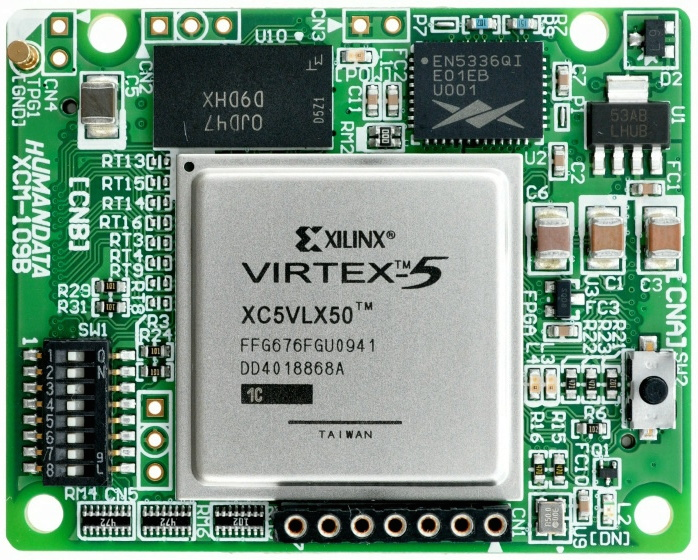
\includegraphics[width=0.45\textwidth]{02_pulse_formation/pics/fpga} \label{fig:fpga}} & 
\subfloat[ASIC~\cite{ASIC:00000}]{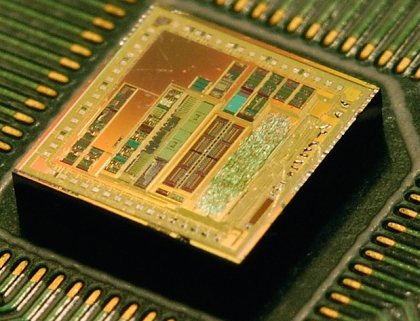
\includegraphics[width=0.45\textwidth]{02_pulse_formation/pics/asic}  \label{fig:asic}}
\end{tabular}
\caption{An example of an FPGA and an ASIC chip}
\end{figure}
